\documentclass{article}

% Packages required to support encoding
\usepackage{ucs}
\usepackage[utf8x]{inputenc}
\usepackage{graphicx} 
% Packages required by code

% Packages always used
\usepackage{listings}
\usepackage{hyperref}
\usepackage{xspace}
\usepackage[usenames,dvipsnames]{color}
\hypersetup{colorlinks=true,urlcolor=blue}


\usepackage[framed,numbered,autolinebreaks,useliterate] {mcode}


\usepackage{geometry}
\geometry{letterpaper,textwidth=350pt,textheight=680pt,tmargin=60pt,
            left=72pt,footskip=24pt,headsep=18pt,headheight=14pt}
\usepackage{amsmath}
\usepackage{amssymb}
\usepackage{textcase}
\usepackage{soul}

\newcommand{\mat}[1]{\boldsymbol{#1}}\renewcommand{\vec}[1]{\boldsymbol{\mathrm{#1}}}
\newcommand{\vecalt}[1]{\boldsymbol{#1}}

\newcommand{\conj}[1]{\overline{#1}}

\newcommand{\normof}[1]{\|#1\|}
\newcommand{\onormof}[2]{\|#1\|_{#2}}

\newcommand{\itr}[2]{#1^{(#2)}}
\newcommand{\itn}[1]{^{(#1)}}

\newcommand{\eps}{\varepsilon}
\newcommand{\kron}{\otimes}

\DeclareMathOperator{\diag}{diag}
\DeclareMathOperator{\trace}{trace}
\DeclareMathOperator{\tvec}{vec}

\newcommand{\prob}{\mathbb{P}}
\newcommand{\probof}[1]{\prob\left\{ #1 \right\}}

\newcommand{\pmat}[1]{\begin{pmatrix} #1 \end{pmatrix}}
\newcommand{\bmat}[1]{\begin{bmatrix} #1 \end{bmatrix}}
\newcommand{\spmat}[1]{\left(\begin{smallmatrix} #1 \end{smallmatrix}\right)}
\newcommand{\sbmat}[1]{\left[\begin{smallmatrix} #1 \end{smallmatrix}\right]}

\newcommand{\RR}{\mathbb{R}}
\newcommand{\CC}{\mathbb{C}}

\providecommand{\eye}{\mat{I}}
\providecommand{\mA}{\ensuremath{\mat{A}}}
\providecommand{\mB}{\ensuremath{\mat{B}}}
\providecommand{\mC}{\ensuremath{\mat{C}}}
\providecommand{\mD}{\ensuremath{\mat{D}}}
\providecommand{\mE}{\ensuremath{\mat{E}}}
\providecommand{\mF}{\ensuremath{\mat{F}}}
\providecommand{\mG}{\ensuremath{\mat{G}}}
\providecommand{\mH}{\ensuremath{\mat{H}}}
\providecommand{\mI}{\ensuremath{\mat{I}}}
\providecommand{\mJ}{\ensuremath{\mat{J}}}
\providecommand{\mK}{\ensuremath{\mat{K}}}
\providecommand{\mL}{\ensuremath{\mat{L}}}
\providecommand{\mM}{\ensuremath{\mat{M}}}
\providecommand{\mN}{\ensuremath{\mat{N}}}
\providecommand{\mO}{\ensuremath{\mat{O}}}
\providecommand{\mP}{\ensuremath{\mat{P}}}
\providecommand{\mQ}{\ensuremath{\mat{Q}}}
\providecommand{\mR}{\ensuremath{\mat{R}}}
\providecommand{\mS}{\ensuremath{\mat{S}}}
\providecommand{\mT}{\ensuremath{\mat{T}}}
\providecommand{\mU}{\ensuremath{\mat{U}}}
\providecommand{\mV}{\ensuremath{\mat{V}}}
\providecommand{\mW}{\ensuremath{\mat{W}}}
\providecommand{\mX}{\ensuremath{\mat{X}}}
\providecommand{\mY}{\ensuremath{\mat{Y}}}
\providecommand{\mZ}{\ensuremath{\mat{Z}}}
\providecommand{\mLambda}{\ensuremath{\mat{\Lambda}}}
\providecommand{\mPbar}{\bar{\mP}}

\providecommand{\ones}{\vec{e}}
\providecommand{\va}{\ensuremath{\vec{a}}}
\providecommand{\vb}{\ensuremath{\vec{b}}}
\providecommand{\vc}{\ensuremath{\vec{c}}}
\providecommand{\vd}{\ensuremath{\vec{d}}}
\providecommand{\ve}{\ensuremath{\vec{e}}}
\providecommand{\vf}{\ensuremath{\vec{f}}}
\providecommand{\vg}{\ensuremath{\vec{g}}}
\providecommand{\vh}{\ensuremath{\vec{h}}}
\providecommand{\vi}{\ensuremath{\vec{i}}}
\providecommand{\vj}{\ensuremath{\vec{j}}}
\providecommand{\vk}{\ensuremath{\vec{k}}}
\providecommand{\vl}{\ensuremath{\vec{l}}}
\providecommand{\vm}{\ensuremath{\vec{l}}}
\providecommand{\vn}{\ensuremath{\vec{n}}}
\providecommand{\vo}{\ensuremath{\vec{o}}}
\providecommand{\vp}{\ensuremath{\vec{p}}}
\providecommand{\vq}{\ensuremath{\vec{q}}}
\providecommand{\vr}{\ensuremath{\vec{r}}}
\providecommand{\vs}{\ensuremath{\vec{s}}}
\providecommand{\vt}{\ensuremath{\vec{t}}}
\providecommand{\vu}{\ensuremath{\vec{u}}}
\providecommand{\vv}{\ensuremath{\vec{v}}}
\providecommand{\vw}{\ensuremath{\vec{w}}}
\providecommand{\vx}{\ensuremath{\vec{x}}}
\providecommand{\vy}{\ensuremath{\vec{y}}}
\providecommand{\vz}{\ensuremath{\vec{z}}}
\providecommand{\vpi}{\ensuremath{\vecalt{\pi}}}

\sodef\allcapsspacing{\upshape}{0.15em}{0.65em}{0.6em}%

\makeatletter
\def\maketitle{%
\par
\hrule height 0.75pt\vspace{1ex}
\par\noindent
\begin{minipage}{0.5\textwidth}
\scshape
purdue university $\cdot$ CS 580 \\
Introduction to the Analysis of Algorithms
\end{minipage}
\begin{minipage}{0.5\textwidth}
\raggedleft
\MakeTextUppercase{\allcapsspacing{\@title}}\\[0.2ex]
\textit{\@author}\\[0.2ex]
\textit{\@date}
\end{minipage}
\par\vspace{1ex}
\hrule height 1pt
\vspace{2ex}
\par
}
\makeatother

\author{Jun Cheng}
\title{Lecture Notes}
% auto generate a title
\AtBeginDocument{\maketitle}


\title{Homework}



\begin{document} 



\hypertarget{problem_0_homework_checklist_2}{}
\subsection*{{Problem 0: Homework checklist}}
\label{problem_0_homework_checklist_2}

\checkmark	I didn't talk with any one about this homework. \newline
\checkmark 	Source-code are included at the end of this document. 


\hypertarget{problem_1_prove_or_disprove_3}{}
\subsection*{{Problem 1: Prove or disprove}}
\label{problem_1_prove_or_disprove_3}

For the proof below, I will assume all the matrices are $n\times n$ square matrices.                                                                

\begin{enumerate}%       

\item The product of two diagonal matrices is diagonal. \newline
$\mA $  and  $\mB $ are diagonal matrices, so \newline 
$\mA_{ij}= 0, if \ i\neq j $  \newline
$\mB_{ij}= 0, if \ i\neq j $  \newline
$\mC = \mA\times\mB$ \newline
$\mC_{ij}=\sum_{k=1}^{n}{\mA_{ik}\mB_{kj}} $\newline
Only if $i=j=k$, $\mC_{ij} $ will not be zero, which mean $\mC$ is also a diagonal matrix. 

\item The product of two upper triangular matrices is upper triangular
$\mA $  and  $\mB $ are two upper triangular matrices, so \newline 

$\mA_{ij}= 0, if  \ i \geqslant j $  \newline
$\mB_{ij}= 0, if \ i\geqslant j $  \newline
$\mC = \mA\times\mB$ \newline
$\mC_{ij}=\sum_{k=1}^{n}{\mA_{ik}\mB_{kj}} $\newline
When $i\geqslant j $, $\mC_{ij}=0 $ because one of $\mA_{ik} $ and $\mB_{kj} $ must be zero. 



\item The product of two symmetric matrices is symmetric.
$\mA $  and  $\mB $ are two symmetric matrices, so \newline 

$\mA_{ij}= \mA_{ji} , if \  i = j $  \newline
$\mB_{ij}= \mB_{ji} , if\  i = j $  \newline
$\mC = \mA\times\mB$ \newline
$\mC_{ij}=\sum_{k=1}^{n}{\mA_{ik}\mB_{kj}} $\newline
Then $\mC_{ij} $ is not necessary to be equal to $\mC_{ji} $\newline
Counter-example: \newline
$\mA=\bmat{1&1\\1&2}$ is a symmetric matrix; \newline
$\mB=\bmat{1&1\\1&1}$ is also a symmetric matrix.\newline
$\mC = \mA\times\mB = \bmat{2&2\\3&3} $ which is not a symmetric matrices.  \newline


\item The product of two orthogonal matrices is orthogonal.

\item The product of two square, full rank matrices is full rank
This statement is incorrect. \\
Counter-example:\\
$\mA=\bmat{1&1\\1&2}$ is a full rank matrix; \newline
$\mB=\bmat{3&5\\1&1}$ is also a full rank matrix.\newline
$\mC = \mA\times\mB = \bmat{4&6\\2&3} $ which is not a full matrices.  \newline


\end{enumerate} 

\hypertarget{problem_2_prove_or_disprove_3}{}
\subsection*{{Problem 2}}
\label{problem_2_prove_or_disprove_3}
We know $\mU$ and $\mV$ are square orthogonal matrices, then
\begin{align}
\mU^T\mU=\mI,  \mV^T\mV=\mI 
\end{align}
$\|\mU\mA\mV\|_2^2
=\mV^T\mA^T\mU^T\mU\mA\mV \\
= \mV^T\mA^T\mA\mV \\
= \mV^T\|\mA\|_2^2\mV \\
=\mV^T\mV\|\mA\|_2^2 \\
=\|\mA\|_2^2 \\$
Therefore $\|\mA\|_2 $ is orthogonally invariant. \\

\hypertarget{problem_3_prove_or_disprove_3}{}
\subsection*{{Problem 3}}
\label{problem_1_prove_or_disprove_3}

\begin{align} 
f(\mA) = \max_{i,j}|A_{ij}| 
\end{align} 

\begin{enumerate} 

\item 
\begin{itemize}
\item  $f(A)>0, when \mA\neq0, \\ f(A)=0\ iff \mA=0 $
\item For and scalar $k$, \\  $ f(k\mA) \\= \max_{i,j}|kA_{ij}| \\= k\max_{i,j}|A_{ij}| \\=kf(\mA)$
\item
$f(\mA+\mB) \\
=\max_{i,j}|A_{ij}+B_{ij}| \\ 
\leq \max_{i,j}|A_{ij}| + \max_{i,j}|B_{ij}| \\
=f(\mA) + f(\mB)$
\end{itemize}
Therefore $f(\mA)$is a matrix norm. 
\item 
$f(\mA\mB) \\
=\max_{i,j}|A_{ij}B_{ij}|\\ 
\leq \max_{i,j}|A_{ij}|  \max_{i,j}|B_{ij}| \\
=f(\mA)f(\mB)$

The $\leq$ is not necessary to be.  A counter example: \\
$\mA= \bmat{3 &3\\3&3} \\
\mB= \bmat{3&3\\3&3} \\ 
\mA\mB= \bmat{18&18\\18&18} $\\
$f(\mA) = 3 \\ 
f(\mB) = 3 $\\
f(\mA\mB) = 18 \\
Then $ f(\mA\mB) > f(\mA)f(\mB)  $\\
So $f$ does not satisfy the sub-multiplicative property. 

\item 
\begin{align} 
g(\mA) = \sigma f(\mA) 
\end{align}
$g(\mA\mB) =\sigma \max_{i,j}|A_{ij}B_{ij}|\\ 
g(\mA)g(\mB) =\sigma^2\max_{i,j}|A_{ij}|  \max_{i,j}|B_{ij}|\\$\\
To make 
\begin{align} 
g(\mA\mB) \leq g(\mA)g(\mB) \\
\sigma \max_{i,j}|A_{ij}B_{ij}| \leq \sigma^2\max_{i,j}|A_{ij}|  \max_{i,j}|B_{ij}| \\
\sigma \geq\frac{\max_{i,j}|A_{ij}B_{ij}|}{\max_{i,j}|A_{ij}|  \max_{i,j}|B_{ij}|} 
\end{align}

Therefore there exists $\sigma>0$ such that: $g(\mA)=\sigma f(\mA) $
\end{enumerate} 


\hypertarget{problem_4_prove_or_disprove_3}{}
\subsection*{{Problem 4}}
\label{problem_4_prove_or_disprove_3}
\begin{align}
f(x)=\|x\vk^T\|
\end{align}

\begin{enumerate}
\item 
\begin{itemize} 
	\item  $f(x)>0, when \mA\neq0, \\ f(x)=0\ iff \mA=0 $ because $\|\mA\| $is a matrix norm. 
	\item  $f(mx) = \|mx\vk^T\| =m\|x\vk^T\| = mf(x) $ 
	\item $f(x+y) = \|(x+y)\vk^T\| = \|x\vk^T+y\vk^T\| \leq \|x\vk^T\|+\|y\vk^T\| = f(x)+f(y)$
\end{itemize}
Therefore $f$ is a vector norm. 

\item If $\|\mA\|$ is a sub-multiplicative matrix norm, 
\begin{align}
f(\mA x)=\|\mA x\vk^T\| \leq \|\mA\| \|x\vk^T\| = \|\mA\| f(x) 
\end{align}
\end{enumerate}


\hypertarget{problem_5_prove_or_disprove_3}{}
\subsection*{{Problem 5  (Choice 1) }}
\label{problem_5_prove_or_disprove_3}


$f(\vx)$ = sum of two largest entries in $\vx$ by absolute value is a vector form. \\
Suppose
\begin {gather*}
\vx=\bmat{x_1\\ x_2\\ x_3}  
\end{gather*}  
Then the unit-ball should include all points which satisfy conditions:  
\begin {gather*}
|x_1|+|x_2|= 1, |x_3|\leq |x_1| , \  |x_3|\leq|x_2|\\
|x_2|+|x_3|= 1, |x_1|\leq |x_2| , \  |x_3|\leq|x_3|\\
|x_3|+|x_1|= 1, |x_2|\leq |x_3| , \  |x_3|\leq|x_1|
\end{gather*}  
I used Monte Carlo method to generate $N=300000 $ points which satisfy those conditions, as shown ind Figure 1. 
\begin{figure}
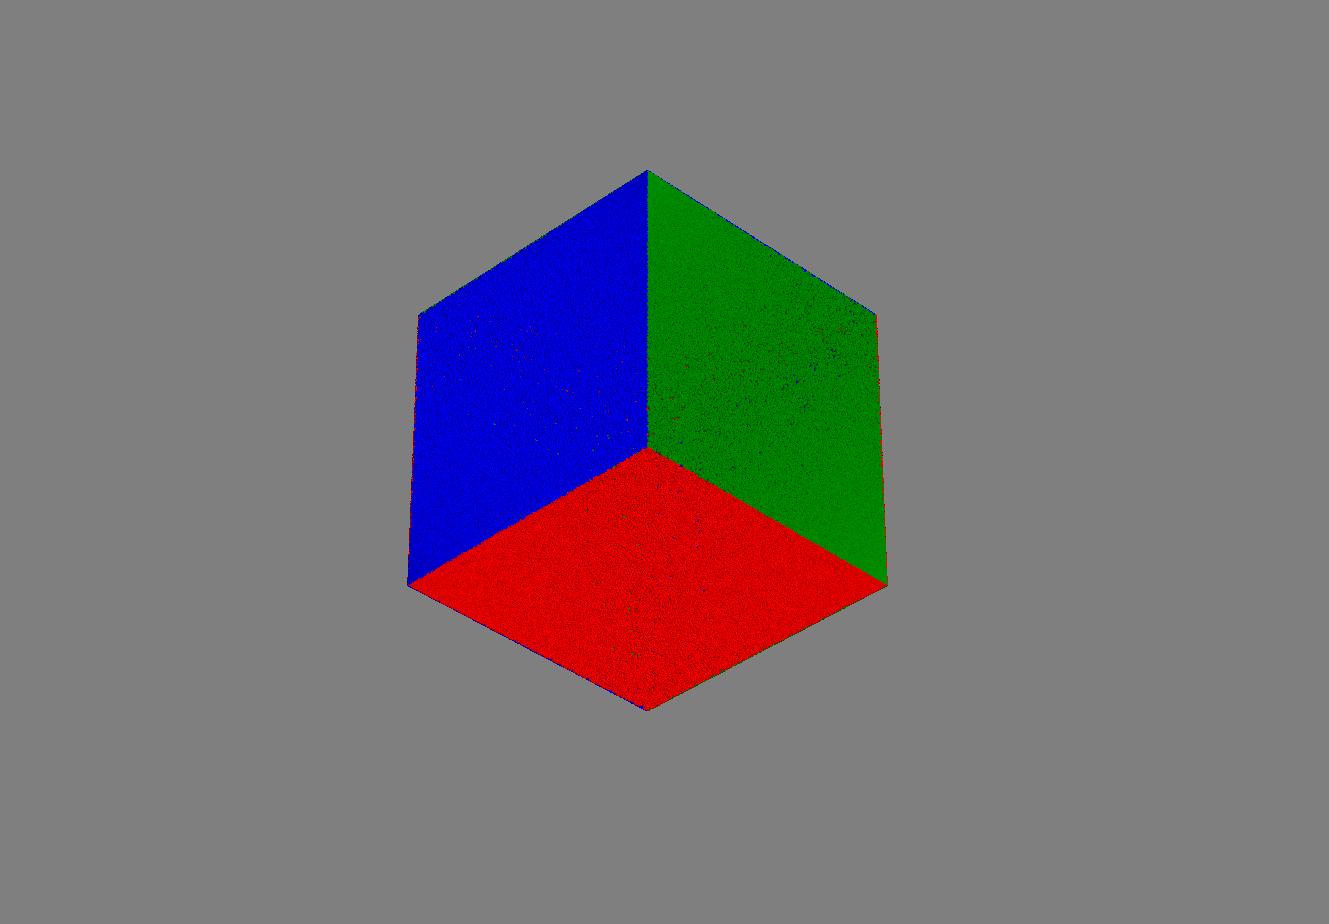
\includegraphics[width=0.6\textwidth]{figure1}
\centering
\end{figure} 

\begin{figure}
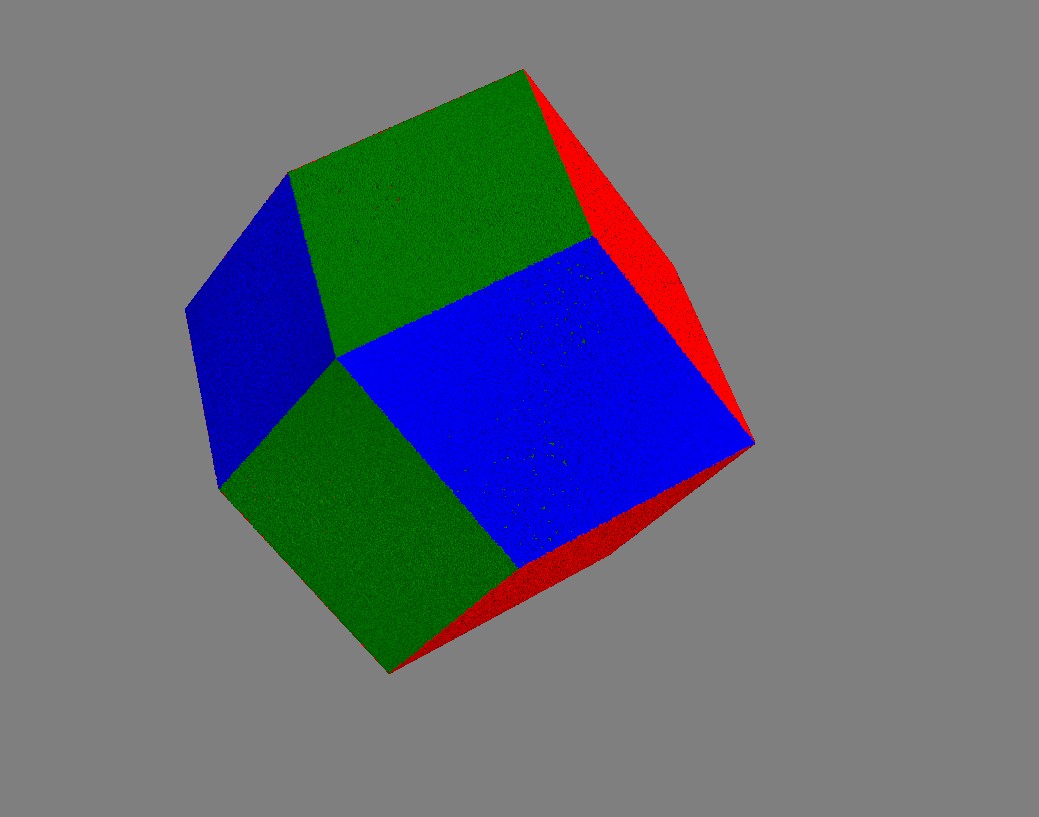
\includegraphics[width=0.6\textwidth]{figure2}
\centering
\end{figure} 

\begin{figure}
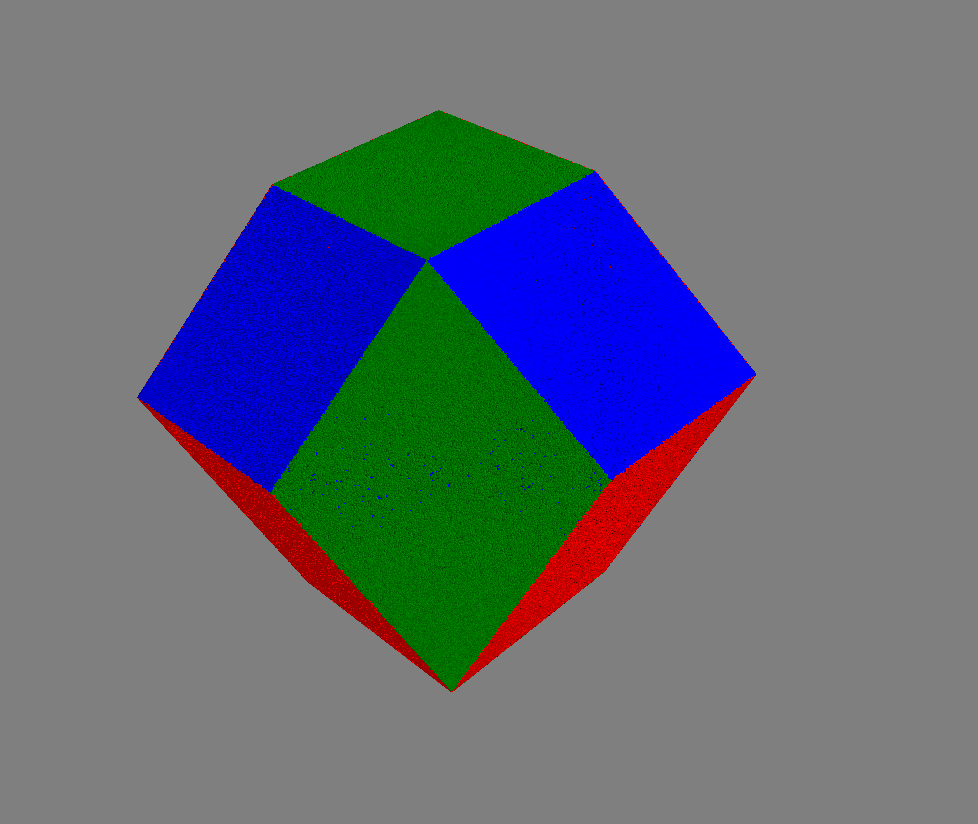
\includegraphics[width=0.6\textwidth]{figure3}
\centering
\end{figure} 

\begin{figure}
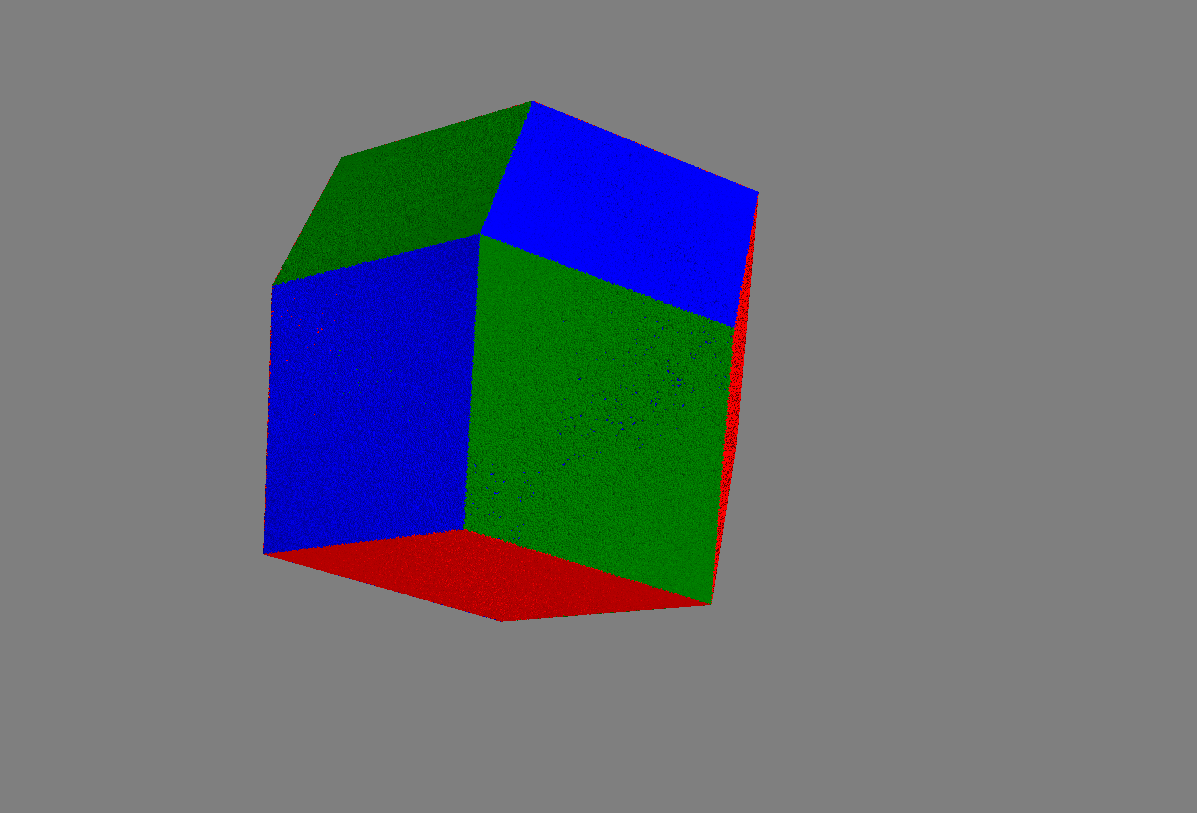
\includegraphics[width=0.6\textwidth]{figure4}
\centering
\caption{The unit-ball surface from different views. Color images are in electronic version.}
\end{figure} 

\end{document}



















